\section{Development history and negative results}\label{secA2}
The hybrid model was the third design we evaluated. We report the two earlier designs and the selection steps that led from one to the next, because the negative results are informative and because the final configuration was chosen from among them. Throughout, choices were made on source validation AUROC only, with Georgia held out and seed 0, and test metrics were not used to choose a configuration.

\subsection{Design v1: text-only head with teacher pseudo-labels}\label{secA2:v1}
The first design used the text-anchored label-query head of Section~\ref{sec:head} as the only head, and trained it with the masked asymmetric loss, implication completion, MixStyle and confidence-gated \emph{hard} pseudo-labels from an exponential-moving-average teacher on unobserved entries of seen diagnoses (threshold 0.9 for positives and 0.05 for negatives, weight ramped linearly to 0.5 over the first 30\% of training, teacher momentum 0.999 without warm-up). The student was validated, selected and tested. Table~\ref{tab:v1} reports this design and seven single-seed ablations of it under leave-one-database-out, together with the baselines in the same conditions (no weight averaging, seed 0).

\begin{table}[!htbp]
\centering\footnotesize
\caption{Design v1 (text-only head with hard teacher pseudo-labels) and its ablations, seed 0, no weight averaging, compared with the baselines under the same conditions: seen-diagnosis macro AUROC averaged over the four held-out databases, and macro AUROC on the five unseen Shaoxing--Ningbo diagnoses ($\times100$).}\label{tab:v1}
\begin{tabular}{lcc}
\toprule
Configuration & Seen AUROC & Unseen AUROC (S--N) \\
\midrule
\multicolumn{3}{l}{\emph{Baselines (linear head, seed 0, no weight averaging)}} \\
Naive pooling & 83.98 & 53.1 \\
Masked loss & 85.19 & 50.0 \\
Li-style & 85.44 & 50.9 \\
CORAL & 85.27 & 51.0 \\
DANN & 85.04 & 53.7 \\
GroupDRO & 84.89 & 52.6 \\
MixStyle & 85.33 & 50.8 \\
\midrule
\multicolumn{3}{l}{\emph{Design v1 and its ablations}} \\
v1 (full) & 84.32 & 66.2 \\
$-$ pseudo-labels (masked loss only) & 85.31 & 68.0 \\
$-$ implication completion & 85.67 & 69.0 \\
$-$ MixStyle & 85.22 & 71.3 \\
learned queries instead of text anchors & 85.02 & 51.2 \\
name-only descriptions & 84.82 & 64.6 \\
general-domain text encoder (MPNet) & 84.94 & 67.8 \\
linear head with pseudo-labels (no text head) & 85.37 & 50.9 \\
\bottomrule
\end{tabular}
\end{table}

Three findings shaped the subsequent designs. First, text anchoring is what makes unseen diagnoses scorable: replacing the anchors by learned queries in the same decoder, or the text head by a linear head, reduces unseen-diagnosis AUROC to chance (51.2 and 50.9), whereas every text-anchored variant scores them between 64.6 and 71.3. The description matters: bare names lose 1.6 points relative to full descriptions, and a general-domain encoder is comparable to the biomedical one. Second, the full v1 design was the weakest text-anchored variant on seen diagnoses, and removing \emph{any one} of pseudo-labels, implication completion or MixStyle improved it by about one point. Third, its validation AUROC dropped abruptly on all four folds once pseudo-labels took effect, by 7 to 31 points, and recovered only partially by the end of training (Fig.~\ref{fig:curves}a).

\begin{figure}[!htbp]
\centering
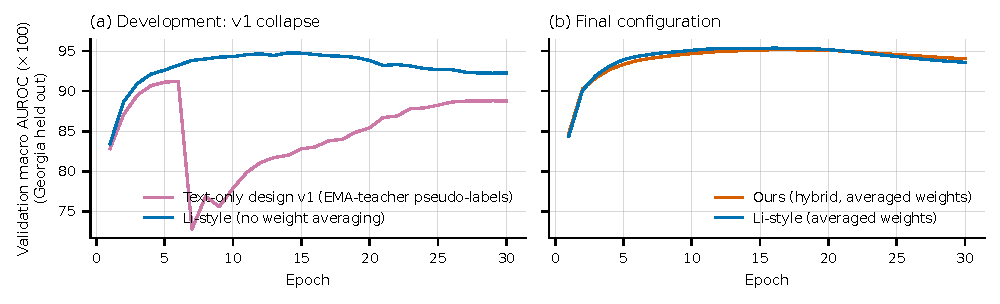
\includegraphics[width=\textwidth]{generated/fig_curves.pdf}
\caption{Validation macro AUROC per epoch with Georgia held out. (a) Design v1 collapses when pseudo-labels take effect (epoch 7), whereas the Li-style baseline trained identically without pseudo-labels does not. (b) The final hybrid configuration and the Li-style baseline, both with weight averaging (seed 1), train smoothly and select a checkpoint around epoch 15.}\label{fig:curves}
\end{figure}

\paragraph{Diagnosis of the collapse.}
Inspection of the logged pseudo-label statistics identified three interacting causes. (i) Hard pseudo-labels were biased towards positives on diagnoses whose implication parent is completed: implication completion (Eq.~\eqref{eq:rules}) creates parent columns that are observed only when positive, so the model learns high parent probabilities, and the teacher then turns unobserved parent entries into confident positive pseudo-labels, which feed back into the student. (ii) With a constant momentum of 0.999 and no warm-up, the teacher still contained $0.999^{t}$ of its random initialization after $t$ steps, about 20\% when pseudo-labels began to take effect, so early pseudo-labels came from a partly random network. (iii) Hard thresholds turned small teacher biases into full-weight targets. These causes are specific to pseudo-labeling and implication completion, which is consistent with the ablations in which removing either one improved seen-diagnosis accuracy.

\subsection{Design v2: corrected text-only head}\label{secA2:v2}
The second design kept a single text-anchored head and corrected each cause: soft rather than hard pseudo-targets, applied from the end of the learning-rate warm-up; implication used as a label-free consistency constraint (the probability of a parent should not be lower than that of its child) instead of positive-only completed targets; the momentum warm-up of Eq.~\eqref{eq:ema}; and validation, selection and testing of the averaged weights. Because a pure text head lacks the per-diagnosis capacity of a linear head, a class-specific residual for seen diagnoses was also evaluated: a per-diagnosis bias, a per-diagnosis read-out of the diagnosis' own cross-attended evidence, a per-diagnosis read-out of the pooled tokens, or both read-outs. Unseen diagnoses keep the pure text logit. Table~\ref{tab:sweeps} (top) reports the four candidates and two zero-shot proxies, in which five diagnoses annotated by PTB-XL and Shaoxing--Ningbo were withheld from training and scored on the validation split. The configuration with both read-outs (S1) was selected by the pre-registered rule; with three seeds on all folds it reached 85.66 (Table~\ref{tab:ablation}, ``text head only''), above v1 but still 0.6 points below the masked and Li-style baselines with weight averaging. The collapse was eliminated, but a single text-anchored head, even with a class-specific residual, did not reach the seen-diagnosis accuracy of a linear head.

\begin{table}[!htbp]
\centering\footnotesize
\caption{Configuration sweeps on one fold (Georgia held out, seed 0). Selection used the source validation macro AUROC only; ``zero-shot proxy'' is the validation macro AUROC on five diagnoses withheld from training, at the selected epoch. The reference is Li-style with weight averaging on the same fold (validation 95.31).}\label{tab:sweeps}
\begin{tabular}{llcc}
\toprule
 & Configuration & Validation AUROC & Zero-shot proxy \\
\midrule
\multicolumn{4}{l}{\emph{v2 sweep (text-only head)}} \\
S1 & both residual read-outs, averaged weights & \textbf{94.56} & 68.6 \\
S2 & as S1, student weights & 94.12 & -- \\
S3 & query read-out only, averaged weights & 94.37 & -- \\
S4 & no residual, averaged weights & 93.90 & 67.9 \\
\midrule
\multicolumn{4}{l}{\emph{Hybrid sweep (linear head + text head)}} \\
H1 & linear scoring of seen diagnoses & 95.19 & -- \\
H2 & mean-probability fusion (selected) & \textbf{95.27} & 69.9 \\
H3 & as H2, detached text head & 95.33 & 66.4 \\
H4 & as H2, with soft pseudo-labels & 95.23 & -- \\
\bottomrule
\end{tabular}
\end{table}

\subsection{Design v3: hybrid head}\label{secA2:hybrid}
The final design keeps the linear head of the baselines unchanged and adds the pure text-anchored head on the same encoder, as described in Section~\ref{sec:head}. Four variants were compared (Table~\ref{tab:sweeps}, bottom). The pre-registered rule was: highest validation AUROC, with ties within 0.001 broken in favour of the simpler configuration in the order H1 $<$ H2 $<$ H3 $<$ H4, and the zero-shot proxy of the selected configuration checked against that of the detached variant. H3 had the highest validation AUROC but was within 0.001 of H2, which is simpler (it needs no gradient stopping) and had the higher zero-shot proxy (69.9 against 66.4); H2 was therefore selected. H2 did not exceed the Li-style reference on validation (95.27 against 95.31). For this case the rule contained a fallback: H1 was to be chosen if its zero-shot proxy passed a guard (at least 65.9, i.e.\ 2 points below the pure text head of v2) and its validation AUROC was within 0.002 of the reference, so that the claim would rest on the seen-diagnosis performance of the linear head plus the zero-shot ability of the text head. H1 met both conditions (95.19, proxy 69.9). \emph{We did not apply this fallback} and kept H2 as the main configuration; we report the deviation here. Both configurations were subsequently run on all folds with three seeds, H1 as ablation (i) of Table~\ref{tab:ablation}, so the reader can evaluate either choice: H1 has a mean seen-diagnosis AUROC of 86.06 (0.21 below Li-style) and the same unseen-diagnosis AUROC as H2 (67.3 against 67.0), and H2 has 86.57. Had H1 been reported as the main method, the conclusions on unseen diagnoses would be unchanged, and the seen-diagnosis conclusion would be that the method is slightly below, rather than level with, the strongest baselines.

\subsection{Effect of weight averaging}\label{secA2:ema}
Validating, selecting and testing the averaged weights (Eq.~\eqref{eq:ema}) is a generic change that any method can use. Fig.~\ref{fig:ema} compares each baseline with and without it (seed 0, mean over the four held-out databases). It improved every baseline, by 0.33 (DANN) to 1.79 points (naive pooling), and narrowed the spread between baselines. All comparisons in the main text therefore use weight averaging for every method; without it, the baselines would have been 0.3--1.8 points weaker and the advantage of the proposed method correspondingly overstated.

\begin{figure}[!htbp]
\centering
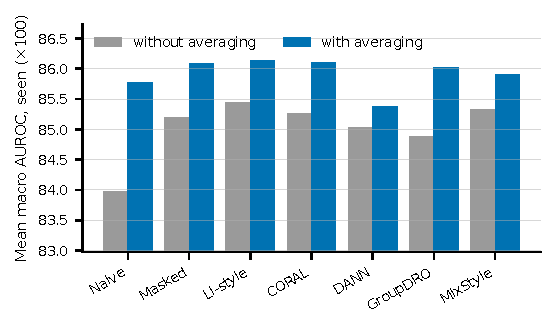
\includegraphics[width=0.62\textwidth]{generated/fig_ema.pdf}
\caption{Seen-diagnosis macro AUROC of each baseline with and without weight averaging (seed 0, mean over four held-out databases).}\label{fig:ema}
\end{figure}
